\par Rating influence people choice on choosing products. Higher rating products have more tendency to be bought. It’s obvious that the relation between rating and the tendency is monotonic: the higher rating is, the more likely it would be bought.We observed that the difference of 4-star and 5-star produce less impact than the difference of 1-star and 2-star rating. So it's reasonable to consider that popularity is correlated to the logarithmic scale of rating. We hereby use $log_5$(rating) with linear relation with some constant $k$. Since the product of the same category has similar usability, so the constant $k$ of the same category might be the same value, defined as $\lambda$ $_{category}$. So we can define $f$ as
\newline

\begin{definition}
$f$(rating)$\ \ \equiv\ \lambda_{category}\ log_5$(rating).
\end{definition}

From the assumption(8), the value of $\lambda$ $_{category}$ can be considered as $1$.

Therefore, we can have that 
\begin{center}
    $Q'_{2,product}=f$(rating)$Q_{2,product}$
\end{center}

\par 
It’s reasonable to have brand's influence factor in the model of demand of the product, since brand loyalty influence how buyer will choose the product. According to the definition of the price elastic of demand change of the particular product($Cd_{product}$) which is the percentage of change of the sales due to the change of the price of particular product and the assumption (5),(6),(7), we can conclude that 
\begin{center}
    $Cd_{product}=g$(brand) $Ed_{product type}$
\end{center}
But it is impossible to find the exact value of $Ed_{product type}$ from the stat. Because of the assumption(5), so we assume $Ed_{product type}=-1$. Unfortunately $g$ can’t be define from the given information, we now assume that no brands gain advantages from old clients. So we have 
\begin{definition}
$g$(brand)$\ \ \equiv\ 1.$ 
\end{definition}

As we assume that the $Q_{1,product}$ is the quantity that customer will buy in the usual event.
\par From the price elastic of demand formula and the assumption(7),

\begin{center}
    $Cd_{product}=(\dfrac{Q_{1,product}-Q_{2,product}}{P_{1,product}-P_{2,product}})(\dfrac{P_{1,product}+P_{2,product}}{Q_{1,product}+Q_{2,product}})$
\end{center}
It's also well known that the sign of $Cd_{product}$ is negative(from the assumption(5)). we get $Q_{2,product}$ as 
\begin{center}
    $Q_{2,product}=\dfrac{2Q_{1,product}}{1+\dfrac{Cd_{product}(P_{1,product}-P_{2,product})}{P_{1,product}+P_{2,product}}}-Q_{1,product}$
\end{center}

Since Rating affect buyers’ behavior
\begin{center}
    $Q'_{2,product}=f$(rating)$Q_{2,product}$
\end{center}
Then we can model the popularity of the product(competitive rate) as the ratio between Expected quantity sold during the event with customer rating concerning($Q'_{2,product}$) and the available quantity of the product($Q_{1,product}$).
\begin{model}
    $P_{product}=\dfrac{Q'_{2,product}}{Q_{1,product}}$
\end{model}


As we want to construct the model to describe the level of damage of each layout of the store. According to the assumption(4), we are going to construct the model to indicate the chaos of the product instead, since damage and chaos are correlated. First, we will define the \emph{store} as the only area that contains the particular item. Each item undergoes different amount of risk to be damaged since the chaos is related to many factors: 
\begin{enumerate}
    \item Popularity(competitive rate) of that product [$P_{product}$]
    \item Density of people struggling for that product at specific part of the store [$D_{product}$]
    \item The cost of that product[regular price $P_{1,product}$] (see assumption (10))
    \item The size of that product [$f_2$(product)]
    \item The durability of that product
\end{enumerate}
From the assumption(3) the durability of the product can be neglected. First, it's obviously true that when there are too many people in the small area, there will be very messy. The more density of people in the effective area (see assumption(2)), the more chaotic the store is. In addition, if the popularity of that product is high, the competitive rate of customer is also high, lead to more Chaos in the system. Therefore, in order to calculate chaos of the store, we assume that the relation between the chaos caused by the store and both popularity and the density of customer is linear. Since the value of each product is different, the damage caused by the product is then relates to the cost of that product. It's also a common sense that the chaos depends directly to the physical size of the product. Finally, we can calculate the chaos caused by the store of the product

\[M \equiv D_{product} \times M_{product,i}\times P_{1,product} \times f_2 (product)\times constant\ of\ the\ correlation\]

Let A represents effective area which already mentioned in assumption(2) and $f_2$ maps product the store sell, to the contribution to mess of the store, determine the size of the product. Let a representative of amount of item the store contain is $q_i$, so $P_{product} \times q_i$ indicate the predicted number of customer that will come to struggle this product. 
\medskip Therefore, $D_{product}=\dfrac{P_{product} \times q_i}{A}$

Then we define $M_{product}$ as 
\begin{definition}
$M_{product} \equiv 1+ \dfrac{M}{M_{sum}}$
\end{definition}
,where $M_{sum}$ is the sum of all M value of all store in the shop.
This make $M_{product}\in (1,2)$

Now we have the $M_{product}$ indicate the chaos value caused by the particular store of product.Now consider the row of store and each store's $M_{product}$. Let the $M_{product,i}$ be it's $M_{product}$. As see in figure 1.
\begin{center}
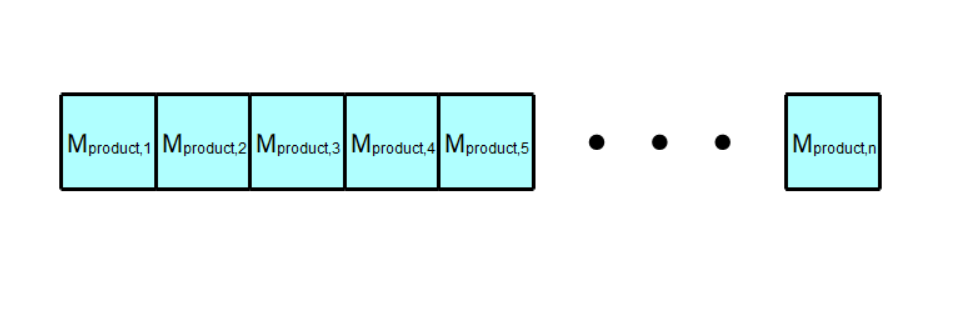
\includegraphics[width=\textwidth]{fig3.PNG}
Figure 1
\end{center}


Since when the store is very mess, it's neighbours will be impacted. So we say that chaos of a walkway that pass through the store is determined by itself and its neighbours Mess. We say that the chaos is the product of itself and its adjacent member because the shoppers don't just increase the messiness to only the store, but to the area(walkway). Chaos of the walk way is formally defined as

\begin{model}
    $C_{path}=\displaystyle{\sum_{i=1}^{n}\ M_{product,i-1}\times M_{product,i}\times M_{product,i+1} }$
\end{model}
,where $M_{product,0}=M_{product,n+1}=1$

Then we define function 
\begin{definition}
$h_2$($M_1,M_n$) $\equiv$ the function that calculate the $C_{pathM_1...M_n}$.
\end{definition}
For instance, the walkway of figure 2 has chaos value $C_{path}$ equal to $[M_1M_2+M_1M_2M_3+M_2M_3M_4+M_3M_4M_5+M_4M_5M_6+M_5M_6]+[M'_1M'_2+M'_1M'_2M'_3+M'_2M'_3M'_4+M'_3M'_4M'_5+M'_4M'_5M'_6+M'_5M'_6]$ and $h_2$($M_1,M_6$)$=[M_1M_2+M_1M_2M_3+M_2M_3M_4+M_3M_4M_5+M_4M_5M_6+M_5M_6]$.In this figure, we use $M_i$ to represent $M_{product,i}$.
\begin{center}
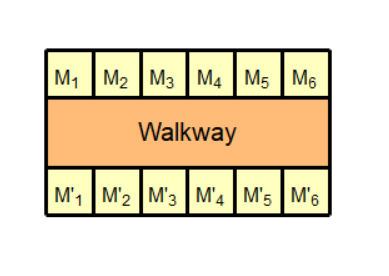
\includegraphics[]{fig1.PNG}

Figure 2.
\end{center}

Next, the mess of the intersection is caused by the shopper walk along the row of store, that is connected to the intersection. The red and green point in the Figure 3 indicate two different types of the intersection. Next we will use $M_{product,i}$ to indicate both chaos value of the product$_i$ and the store that contains p;product$_i$. 

\begin{center}
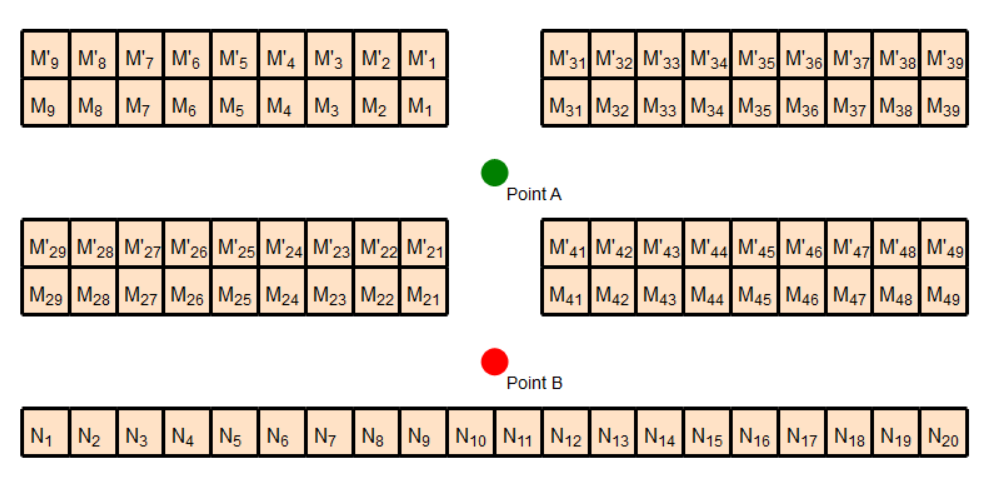
\includegraphics[width=\textwidth]{fig2.PNG}
Figure 3
\end{center}

For the green point, we know that the more people come from 4 directions([$M'_1M_1$ or $M_{31}M'_{31}$], [$M_{31}M_{39}$ or $M'_{41}M'_{49}$], [$M_1M_9$ or $M'_{21}M'_{29}$] and [$M'_{41}M_{41}$ or $M_{21}M'_{21}$]) that connected to this point. So the mess of this intersection point is related to how many shopper come to this point. But customers can only go to this point if customers walk(run) through these 4 walkway. So the chaos of the intersection is directly related to how mess of each store along the walkway. In addition, two products at the corner(adjacent to the intersection) also impact the chaos of the intersection. Because the intersection is where customer will brake, slow down, change the direction, these kind of action can be easily cause the collision of the customer who come from different direction. This collision will affect the store that is adjacent to the intersection. So if these two store which adjacent to the intersection have high value of mess point($M_{product}$), there will be very messy. So we define the function $h_1$(row of store$_i$,intersection$_j$) as the function that calculate the chaos value that generated by the store in the row of store$_i$, which belong to the particular walkway that is connected to the intersection$_j$.
So we define function
\begin{definition}
$h_1$(row  of store$_i$,intersection$_j$)$\equiv \displaystyle{M_{product,1} \times M_{product,2} \times [{\sum_{M_{product,i}\in \mathbb{W}} M_{product,i}}]}$
\end{definition}
\par where $\mathbb{W}$ represent a set of the store in the row of store$_i$ that is connected to the intersection$_j$, the $M_{product,1}$ and $ M_{product,2}$ are adjacent store and the $M_{product,1}$ store connected to the intersection$_j$.

So we define the chaos of the intersection as 

\begin{model}
    $C_{intersection_j}=\displaystyle{\sum_{row\ of\ store_i\in \mathbb{D}}} h_1$(row of store$_i$,intersection$_j$)
\end{model}

Where we define $\mathbb{D}$ as the set of all row of store connected to that intersection$_j$ 

For instance,
\begin{enumerate}
    \item[] $h_1$(row of store$_{M_1...M_9}$,intersection$A$)$=M_1M_2(\sum_{i=1}^{9}M_i)$
    \item[] $C_{intersection_A}=\sum_{i=0}^{3}(M_{i1}M'_{i1}(M_{i1}+M'_{i1})) + M_1M_2(\sum_{i=1}^{9}M_i) + M_{11}M_{12}(\sum_{i=1}^{9}M_{1i}) + M'_{21}M'_{22}(\sum_{i=1}^{9}M'_{2i}) + M'_{31}M'_{32}(\sum_{i=1}^{9}M'_{3i})$
    \item[] $C_{intersection_B}=\sum_{i=2}^{3}(M_{i1}M'_{i1}(M_{i1}+M'_{i1}) + M_{i1}M_{i2}(\sum_{j=1}^{9}M_{ij})) + N_9N_{10}(\sum_{i=1}^{10}N_i) + N_{11}N_{12}(\sum_{i=11}^{20}N_i)$
\end{enumerate}

Finally we calculate the chaos value of the shop's layout by adding all $C_{intersection_j}$ for all intersection$_j$ in the shop's layout. This chaos value of the shop's layout can be used to compare which shop's layout will able to cause the highest damage to the product. The shop with high chaos value will able to cause high damage to the product. So our goal is to find the layout of the shop that can make the chaos value to be the lowest.